%class
	\documentclass{beamer}

%template
	\usetheme{HannoverSalman}
	\setbeamertemplate{navigation symbols}{}
	%\setbeamertemplate{footline}{\centering{\insertframenumber/\insertpresentationendpage}}
	%\setbeamertemplate{footline}{\hspace*{.5cm}\scriptsize{\hfill\insertframenumber\hspace*{.5cm}}} 


%packages
	\usepackage{amsmath, amssymb, graphicx,cancel}
	\usepackage[absolute,overlay]{textpos}
	\usepackage{subfigure}
	\usepackage{caption}\captionsetup{labelformat=empty,labelsep=none}
	\usepackage{geometry}
	\geometry{verbose}
	\usepackage{color}
	\usepackage{xmpmulti}
	\usepackage[3D]{movie15}
	\usepackage{hyperref}
%	\usepackage{bookmark}
	\usepackage[open,openlevel=4,atend]{bookmark}
	%\bookmarksetup{color=blue}
	\usepackage{multirow}
	\usepackage[style=numeric,defernumbers, authoryear]{biblatex}
	%\usepackage[square,sort]{natbib}
	%\usepackage{fancyhdr}%\pagestyle{fancy} 

	
	\hypersetup{bookmarksdepth = 4}


%citations files
	\bibliography{MyCitations}

%logoCSIPCPL
    \setlength{\TPHorizModule}{1mm}
    \setlength{\TPVertModule}{1mm}
    \newcommand{\logoCSIPCPL}
    {
    	\begin{textblock}{1}(100,2) %(100,85)  for bottom
    		\includegraphics[width=1.5cm]{figs/logo_CSIP}
    	\end{textblock}
    	
	\begin{textblock}{1}(117,1) %(117,85)  for bottom
    		\includegraphics[width=1.0cm]{figs/logo_CPL}
    	\end{textblock} 
    }

%logo evolution
    \newcommand{\logoEvolution}
    {    	
	\begin{textblock}{1}(110,1) %(117,85)  for bottom
    		\includegraphics[width=0.65in]{figs/logo_evolution.pdf}
    	\end{textblock} 
    }

%logo Qualcomm
    \newcommand{\logoQualcomm}
    {
    	\begin{textblock}{1}(110,2) %(100,85)  for bottom
    		\includegraphics[width=1.5cm]{figs/logo_qualcomm.jpg}
    	\end{textblock}
    }
%logo Qualcomm (long)
    \newcommand{\logoQualcommllong}
    {
    	\begin{textblock}{1}(0,0) 
    		\includegraphics[width=1.25in]{figs/logo_qualcomm_long.jpg}
    	\end{textblock}
    }

%logo Tech Tower
    \newcommand{\logoTechTower}
    {
    	\begin{textblock}{1}(0,0) 
    		\includegraphics[width=1.25in]{figs/logo_TechTower.jpg}
    	\end{textblock}
    }

%logo tree
    \newcommand{\logoTree}
    {
    	\begin{textblock}{1}(0,0) 
    		\includegraphics[width=1.25in]{figs/logo_tree.jpg}
    	\end{textblock}
    }
%page numbers
    \newcommand{\mypagenum}
    {
    	\begin{textblock}{1}(1,94) 
		{\tiny \color[rgb]{0.2,0.2,1}\insertframenumber} %\insertframenumber,\insertpresentationendpage, \inserttotalframenumber
    	\end{textblock}
    }
%my footnote citation
	\newcommand{\myFootnoteCitation}[2]
	{
		\footnote{\tiny \citeauthor{#1}, \emph{#2}, \citeyear{#1}.}  %\citeauthor{#1}, \citetitle{#1}, #2 \citeyear{#1}.
	}
%my refer to citation
	\newcommand{\mycite}[1]
	{
		\emph{\citeauthor{#1} (\citeyear{#1})}
	}
%my footnote website citation
	\newcommand{\myFootnoteWebsiteCitation}[1]
	{
		\footnote{\tiny \citeauthor{#1}}
	}

\let\thefootnote\relax\footnotetext{Footnotetext without footnote mark}


%section underline
%\newcommand{\tmpsection}[1]{}
%\let\tmpsection=\section
%\renewcommand{\section}[1]{\tmpsection{\underline{#1}}}



%commands
	\newcommand{\likelihood}{p(Z_k| x_k) }						%likelihood
	\newcommand{\prior}{p(x_k)  } 								%prior
	\newcommand{\posterior} {p(x_k| Z_k)}						%posterior
	\newcommand{\prediction} {p(x_k| Z_{k-1})}					%prediction
	\newcommand{\update} {p(x_k|Z_k)}							%update
	\newcommand{\observations} {p(Z_k)}						%observations
	\newcommand{\prevobservations} {p(Z_{k-1})}				%previous observations
	\newcommand{\dxpk} {dx_{k-1}}							%dx_{k-1}
	\newcommand{\ChapKolm}{\int{p(x_k| x_{k-1})p(x_{k-1}|Z_{k-1})} \dxpk} %Chapman Kolmogorov

	%algorithm specific: JPDAF
	\newcommand{\likelihoodJPDAF}{p(Z_k| \chi, m, Z_{k-1}) }		%1. likelihood
	\newcommand{\priorJPDAF}{p(\chi|m, Z^{k-1}} 				%2. prior	
	\newcommand{\observationsJPDAF} {p(Z_k}					%3. observations
	\newcommand{\posteriorJPDAF} {p(\chi| Z_k)}					%4. posterior

%environments
	\newenvironment{changemargin}[2]
	{
	  	\begin{list}{}
		{
			\setlength{\topsep}{0pt}%
			\setlength{\leftmargin}{#1}%
			\setlength{\rightmargin}{#2}%
			\setlength{\listparindent}{\parindent}%
			\setlength{\itemindent}{\parindent}%
			\setlength{\parsep}{\parskip}%
		}
	  	\item[]
		}
		{\end{list}
	}
%figures

%colors
\definecolor{darkgreen}{rgb}{0,0.5,0}

%personal details
	\author{Salman Aslam}
	\institute{Advisor, Dr Christopher Barnes (ECE)\\Co-advisor, Dr Aaron Bobick (CoC)\\Georgia Institute of Technology}
	\date{}

\begin{document}

%####################################################################################################
\title{Residual Vector Quantization}
%####################################################################################################
\begin{frame}\logoTechTower
	\author{Salman Aslam}
	\titlepage
\end{frame}

\begin{frame}
\frametitle{Outline}
\logoTechTower\logoCSIPCPL
	\setcounter{tocdepth}{1}	
	\tableofcontents
\end{frame}


%######################################################################
\section{INTRODUCTION}
%######################################################################
%====================================
\subsection{\ \ \ \ notation}
%====================================
\begin{frame}
\frametitle{Introduction}
\framesubtitle{notation}
\logoCSIPCPL\mypagenum
	\begin{itemize}\tiny
		\item Dimensions
			\begin{itemize}\tiny
				\item {\color{red}$L$}: scalar, number of input data points
				\item {\color{red}$M$}: scalar, number of templates per stage, $m=0, 1, \ldots M-1$
				\item {\color{red}$P$}: scalar, number of stages, $p=0, 1, \ldots P-1$
				\item {\color{red}$N$}: scalar, dimensionality of input space, i.e. $R^N$
			\end{itemize}
		\item Input data
			\begin{itemize}\tiny
				\item {\color{red}$\mathbf{x}_{p,1}, \mathbf{x}_{p,2}, \ldots \mathbf{x}_{p, L}$}: vectors (column vectors), $L$ $N$-dimensional input data points to $p$-th stage
				\item {\color{red}$\mathcal{X}_p$}: set of above data points
				\item {\color{red}$X_p$}: $N$x$L$ matrix of above data points
%				\item {\color{red}$\mathbf{z}_p$}: Mean removed input data at stage $p$, $\mathbf{z}_p = \{\mathbf{z}_{p_1}, \mathbf{z}_{p_2}, \ldots \mathbf{z}_{p_L}\}$, $\mathbf{z}_p = \mathbf{x}_p - \frac{1}{N}\sum\limits_{i=1}^N \mathbf{x}_{p_i}$
%				\item {\color{red}$Z_p$}: Mean removed input data ($N$x$L$ matrix) at stage $p$, $Z_p = \left[\mathbf{z}_{p_1} \mathbf{z}_{p_2} \ldots \mathbf{z}_{p_L} \right]$
			\end{itemize}
		\item Codevectors
			\begin{itemize}\tiny
				\item {\color{red}$\mathbf{z}_{p, 1}, \mathbf{z}_{p, 2},\ldots \mathbf{z}_{p, M}$}: $M$ $N$-dimensional stage codevectors computed at $p$-th stage
				\item {\color{red}$\mathcal{Z}_p$}: set of above codevectors 
			\end{itemize}
		\item Principal directions
			\begin{itemize}\tiny
				\item {\color{red}$\mathbf{u}_{p,1}, \mathbf{u}_{p,2}, \ldots \mathbf{u}_{p, {M-1}}$}: $M-1$ principal directions that span the cluster centroid subspace at $p$-th stage
			\end{itemize}
		\item Miscellaneous
			\begin{itemize}\tiny
				\item {\color{red}$\delta$}: probability weight given to empty bins in histograms
			\end{itemize}
	\end{itemize}
\end{frame}
% $Z_pZ_p^T\mathbf{u}_{p_k} = \lambda_{p_k} \mathbf{u}_{p_k}$.  The first $M-1$ of these principal directions span the cluster centroid subspace for stage $p$


\begin{frame}
\frametitle{Introduction}
\framesubtitle{notation: other than RVQ}
\logoCSIPCPL \mypagenum
	\begin{itemize}
		\item {\color{red}$q$}: PCA only, number of retained dimensions
		\item {\color{red}$C$}: SVM only, weighting in SVM optimization
		\item {\color{red}$\gamma$}: SVM only, kernel parameter in polynomial, RBF, sigmoid kernels
	\end{itemize}
\end{frame}

%=====================================
\subsection{\ \ \ \ background}
%=====================================
\begin{frame}
\frametitle{Introduction}
\framesubtitle{signal coding}
\logoCSIPCPL \mypagenum
	\value{finalframe}
	\begin{enumerate}
		\item Lossless coding
			\begin{itemize}
				\item consideration: {\color{blue}rate}
				\item lower bound: {\color{red}entropy}
			\end{itemize}
		\vspace{0.1in}
		\item Lossy coding
			\begin{itemize}
				\item considerations: {\color{blue}rate and distortion}
				\item lower bound: {\color{red}rate-distortion function}
			\end{itemize}
	\end{enumerate}
\end{frame}





\begin{frame}[plain]
\frametitle{Introduction}
\framesubtitle{entropy}
\logoCSIPCPL\mypagenum
	\begin{changemargin}{-1.3in}{0in}
		\begin{figure}				
			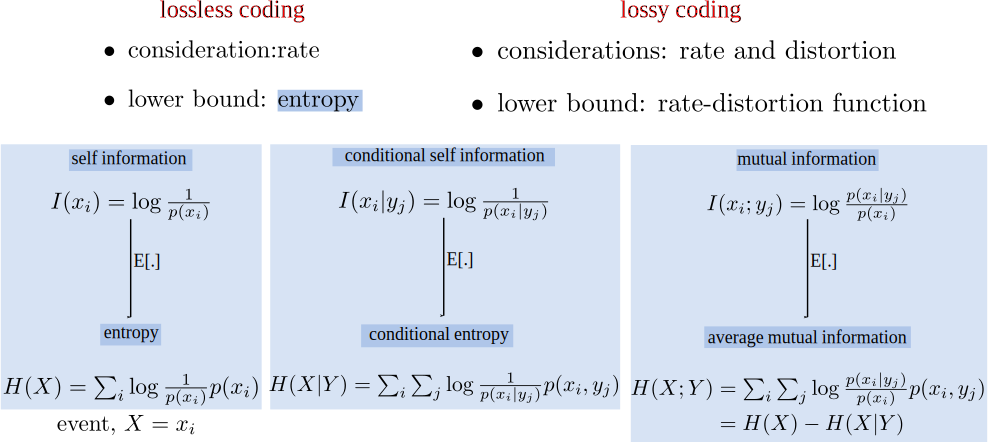
\includegraphics[width=1.3\textwidth]{figs/IT_entropy.pdf}
		\end{figure}
	\end{changemargin}
\end{frame}




\begin{frame}
\frametitle{Introduction}
\framesubtitle{quantization: overview}
\logoCSIPCPL\mypagenum
	{\color{red} Goal: } Data compression
	\begin{itemize}
		\item Minimize some measure of distortion between original and reconstructed data		
		\item Mean squared error (MSE),
			\begin{equation*}
				MSE = \int\limits_{-\infty}^\infty(x - \hat{x})^2f_X(x)dx
			\end{equation*}
	\end{itemize}
\end{frame}


\begin{frame}
\frametitle{Introduction}
\framesubtitle{quantization: overview (cont.)}
\logoCSIPCPL\mypagenum
	For discrete reproduction points, i.e. codevectors, the MSE is,
	\begin{figure}				
		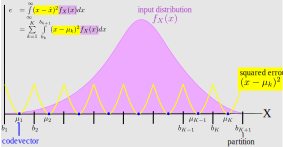
\includegraphics[width=0.9\textwidth]{figs/Quantization_MSE.pdf}
	\end{figure}
\end{frame}



\begin{frame}
\frametitle{Introduction}
\framesubtitle{quantization: block diagram}
\logoCSIPCPL\mypagenum
	\begin{figure}				
		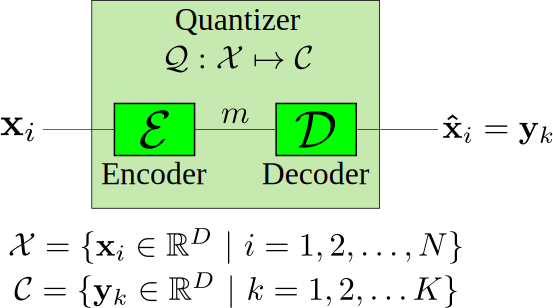
\includegraphics[width=0.9\textwidth]{figs/Quantization_blockDiagram.pdf}
	\end{figure}
\end{frame}




\begin{frame}[plain]
\frametitle{Introduction}
\framesubtitle{Lloyd Max conditions: optimal code-vectors}
\logoCSIPCPL\mypagenum
	\begin{changemargin}{-1.3in}{0in}
		\begin{figure}				
			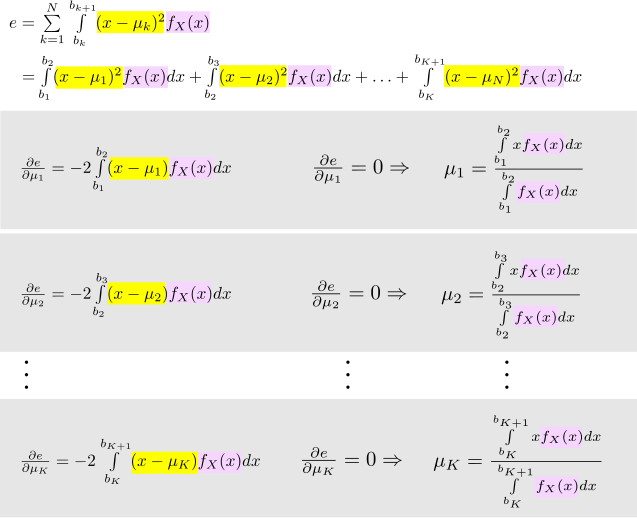
\includegraphics[height=0.8\textheight]{figs/Quantization_optimalCodevectors.pdf}
		\end{figure}
	\end{changemargin}
\end{frame}



\begin{frame}
\frametitle{Introduction}
\framesubtitle{Lloyd Max conditions: optimal partitions}
\logoCSIPCPL\mypagenum
	\begin{figure}				
		\includegraphics[width=1.0\textwidth]{figs/Quantization_optimalPartitions.pdf}
	\end{figure}
\end{frame}



\begin{frame}[plain]
\frametitle{Introduction}
\framesubtitle{Lloyd Max conditions: Optimal partitions (cont.)}
\logoCSIPCPL\mypagenum
	\begin{changemargin}{-1.3in}{0in}
		\begin{figure}				
			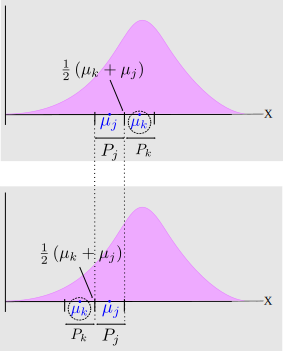
\includegraphics[height=0.8\textheight]{figs/Quantization_optimalPartitions2.pdf}
		\end{figure}
	\end{changemargin}
\end{frame}


\begin{frame}
\frametitle{Introduction}
\framesubtitle{Lloyd Max conditions: summary}
\logoCSIPCPL\mypagenum
	\begin{align*}				
		\frac{\partial{MSE}}{\partial b_j}&=0 \ \ 	\text{for} \ j=1, ... N-1 \\
		\frac{\partial{MSE}}{\partial y_j}&=0 \ \ 	\text{for} \ j=0,1, ... N-1 
	\end{align*}
	\begin{block}{Lloyd-Max conditions}
		\begin{align*}
			b_j = \frac{y_{j-1} + y_j}{2}\\
			y_j=\frac{\int\limits_{b_j}^{b_{j+1}} xf_X(x)dx}{\int\limits_{b_j}^{b_{j+1}} f_X(x)dx}
		\end{align*}
	\end{block}
\end{frame}




\begin{frame}
\frametitle{Introduction}
\framesubtitle{scalar quantization: types\footnote{Sayood, 2005}}
\logoCSIPCPL\mypagenum
	\begin{columns}
		\begin{column}{1.5in}
			\begin{figure}
			{
				\includegraphics[width=0.8\textwidth]{figs/RVQ_midRiseQuantizer}
				\caption {Mid-rise quantizer}
			}
			\end{figure}
		\end{column}
		\begin{column}{1.5in}
			\begin{figure}
			{
				\includegraphics[width=1.0\textwidth]{figs/RVQ_midTreadQuantizer}
				\caption {Mid-tread quantizer}
			}
			\end{figure}
		\end{column}
	\end{columns}
\end{frame}





\begin{frame}
\frametitle{Introduction}
\framesubtitle{scalar quantization: design (method I)}
\logoCSIPCPL\mypagenum
	\begin{itemize}
		\item Start with arbitrary $y_i$ (codevectors)
		\item Hold $y_i$ fixed, compute optimal $b_j$ (partitions)
		\item Hold $b_j$ fixed, compute optimal $y_i$
		\item Algorithm guaranteed to converge
			\begin{itemize}
				\item Distortion is bounded below by 0
				\item For each minimization, distortion is non-increasing
			\end{itemize}
	\end{itemize}
\end{frame}

\begin{frame}
\frametitle{Introduction}
\framesubtitle{vector quantization: overview}
\logoCSIPCPL\mypagenum
	\begin{itemize}
		\item Generalization of scalar quantization
		\item Will always perform better than or equal to scalar quantization
			\begin{itemize}
				\item scalar quantization leads to rectangular cells
				\item VQ can create arbitrary shaped cells
			\end{itemize}		
	\end{itemize}
\end{frame}


\begin{frame}
\frametitle{Introduction}
\framesubtitle{vector quantization: optimal encoder}\logoCSIPCPL\mypagenum
	\vspace{0.2 in}
	{\color{red}Goal}: Given decoder, design encoder 

	\begin{itemize}
		\item Minimize distortion 
			\begin{equation*}	
				d(x,Q(x)) = \min_{y_i} d(x,y_i)
			\end{equation*}
		\item if $y_j$ is unique nearest neigbor of x
			\begin{itemize}
				\item assign x to $R_j$
			\end{itemize}
		\item Choose nearest-neighbor codeword
			\begin{equation*}
				Q(x)=y_i \ \ \text{only if} \ d(x,y_i) \leq d(x,y_j)  \ \forall j
			\end{equation*}
	\end{itemize}

	\begin{figure}
		\includegraphics[width=0.4\textwidth]{figs/RVQ_optimalEncoder}
	\end{figure}
\end{frame}



\begin{frame}
\frametitle{Introduction}
\framesubtitle{vector quantization: optimal decoder}
\logoCSIPCPL\mypagenum
	\vspace{0.2 in}
	{\color{red}Goal}: Given encoder, design decoder 
	\begin{itemize}
		\item centroid
			\begin{equation*}
				y^{\star} = \arg \min_y E[d(x,y) | x \in R]
			\end{equation*}
	\end{itemize}

	\begin{block}{Generalized LLoyd Max conditions}
	\end{block}
\end{frame}



\begin{frame}
\frametitle{Introduction}
\framesubtitle{vector quantization: types}
\logoCSIPCPL\mypagenum
	\begin{itemize}
		\item Unstructured
			\begin{itemize}
				\item Exhaustive Search (ESVQ)
			\end{itemize}
		\item Structured
		\begin{itemize}
			\item Tree Structured (TSVQ)
			\item Transform
			\item Product
				\begin{itemize}
					\item Mean-removed
					\item Shape-gain
					\item Residual (RVQ)
				\end{itemize}
		\end{itemize}
	\end{itemize}
\end{frame}


\begin{frame}
\frametitle{Introduction}
\framesubtitle{vector quantization: TSVQ}
\logoCSIPCPL\mypagenum
	\begin{itemize}
		\item one of the most effective and widely used techniques to reduce search complexity
		\item {\color{red}Design time (training)}
			\begin{itemize}
				\item resulting codebook may not be optimal
				\item however, performance often close to optimal
			\end{itemize}
		\item {\color{red}Run-time (testing)}
			\begin{itemize}
				\item encoding complexity much less than ESVQ
			\end{itemize}
		\item {\color{red}Encoder}
			\begin{itemize}
				\item stage-wise search
			\end{itemize}
		\item {\color{red}Decoder}
			\begin{itemize}
				\item tree-structured codebook only affects search strategy
				\item decoder does not need \textbf{test vectors}
				\item decoder similar to ESVQ
			\end{itemize}
	\end{itemize}
\end{frame}





\begin{frame}
\frametitle{Introduction}
\framesubtitle{vector quantization: design}
\logoCSIPCPL\mypagenum
	\begin{enumerate}
		\item {\color{red}Initialization: Global centroid} 
			\begin{itemize}
				\item find centroid, $y_0$, of entire training set
				\item this is the globally optimal resolution 0 codebook
			\end{itemize}
		\item {\color{red}Splitting}: 
			\begin{itemize}
				\item split $y_0$ into two code words, $y_0$ and $y_0 + \epsilon$
				\item {\color{blue}proportional to eigenvector}: $\epsilon$ can be chosen to be proportional to eigenvector $v$ corresponding to largest eigenvalue $\lambda$ of training set covariance matrix $\Sigma$, or
				\item {\color{blue}proportional to standard deviations, $\sigma_i$}:  make $i$-th component of $\epsilon$ proportional to $\sigma_i$ of dimension $i$ of training set vectors
				\item this new codebook contains previous codebook, and so can be no worse
			\end{itemize}
		\item {\color{red}Optimization}: Run GLA algorithm to produce a good resolution 1 code
		\item {\color{red}Repeat for subsequent stages}: Split all code words in existing resolution $r$ codebook to produce an initial $r+1$ codebook, then optimize it
	\end{enumerate}
\end{frame}


\begin{frame}
\frametitle{Introduction}
\framesubtitle{vector quantization: TSVQ: progressive reconstruction or,\\ successive approximation}
\logoCSIPCPL\mypagenum
	Rather than wait for complete vector,\\
	successively refine as information arrives
	\begin{itemize}
		\item {\color{red}Decoder}
			\begin{itemize}
				\item decoder needs \textbf{test vectors}
			\end{itemize}
	\end{itemize}
\end{frame}



%%%=============================================================
%\subsection{Distortion}
%%%=============================================================
%\begin{frame}\frametitle{Distortion}\logoCSIPCPL\mypagenum
%	\begin{align*}
%		\mathbf{x} &\in R^k \notag\\
%		Q &: R^k \mapsto \mathcal{C}
%	\end{align*}
%			
%	{\color{red}Goal}
%	\begin{itemize}
%		\item codebook (decoder)
%		\item partition (encoder)
%		\item stay as close as possible to the rate distortion curve, i.e. minimize distortion
%		\begin{equation*}
%			D =\sum_i \sum_j d(x_i, y_j) p(x_i,y_j)
%		\end{equation*}
%	\end{itemize}
%\end{frame}


%\begin{frame}[allowframebreaks]
%\frametitle{rate distortion\tiny{\footnote{E. Tuncel, P. Koulgi, and K. Rose, Rate-distortion approach to databases: storage and content-based retrieval," Information Theory, IEEE Transactions on, vol. 50, no. 6, pp. 953-967, 2004}}}
%\framesubtitle{goal}
%\logoCSIPCPL\mypagenum
%	explore relationship between \emph{rate distortion theory} and efficient, content-based data retrieval from high-dimensional databases
%	\begin{itemize}
%		\item These guys study high dimensional databases, search time (rate) vs quality of results (distortion).  Here are some excerpts:
%		\item A highly motivating observation is that the search and retrieval (or indexing) problem bears resemblance to the rate–distortion problem in that it seeks an optimal tradeoff between the amount of data that needs to be read during the search (“rate”) and the quality of the retrieved data in terms of its relevance to the query (“distortion”).
%		\item information-theoretic approaches may offer highly valuable insight into and performance bounds for important problems in storage and retrieval in large databases.
%		\item Moreover, the database context offers a new setting and a variety of problems that would be of interest to researchers in rate–distortion theory
%		\item Similarity search refers to the task of seeking in a database
%the entries that are most similar to a given query object.
%		\item It is in fact impractical
%to store all the extracted feature vectors in a random access
%memory (RAM) and, therefore, it is necessary to read them
%from a hard storage medium, typically a hard disk, during the
%search operation.
%		\item We adopt in this work a widely accepted and very efficient
%approach for approximate similarity searching. Without
%building an indexing mechanism, the search engine simply
%accesses partial information about all the feature vectors.
%		\item In this section, we first derive the rate–distortion region for
%the first layer, i.e., the region of all achievable pairs of query
%processing time and search accuracy.  Next, we derive
%the region of all achievable quadruples .
%Finally, we analyze the conditions for the achievability of
%, where denotes the minimum
%rate needed to achieve search accuracy , and
%denotes the ordinary rate–distortion function at distortion .
%	\end{itemize}
%\end{frame}

%=====================================
\subsection{\ \ \ \ block diagram}
%=====================================
\begin{frame}[plain]
\frametitle{Introduction}
\framesubtitle{block diagram}
\logoCSIPCPL\mypagenum
	\begin{changemargin}{-1.3in}{0in}
		\begin{figure}				
			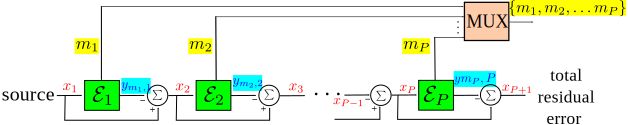
\includegraphics[width=1.3\textwidth]{figs/RVQ_blockDiagram.pdf}
		\end{figure}
	\end{changemargin}
\end{frame}


%====================================
\subsection{\ \ \ \ definitions}
%====================================
\begin{frame}
\frametitle{Introduction}
\framesubtitle{definitions: RVQ}
\logoCSIPCPL\mypagenum
	\begin{itemize}
		\item {\color{red}RVQ} 
			\begin{itemize}
				\item Multi-stage VQs, sequence of small ESVQs
				\item initially perform crude quantization using a small codebook
				\item second quantizer operates on error of first quantizer
				\item third quantizer operates on error of second quantizer, and so on
				\item no reported usage for more than 2 stages, except Prof. Barnes
				\item {\color{blue}direct sum structure} 
					\begin{itemize}
						\item sequential search
						\item linear complexity
					\end{itemize}
			\end{itemize}
	\end{itemize}
\end{frame}



\begin{frame}
\frametitle{Introduction}
\framesubtitle{definitions: optimality}
\logoCSIPCPL\mypagenum
	\begin{itemize}
		\item {\color{red} Optimality}
			\begin{itemize}	
				\item direct application of Lloyd-Max analysis not possible
				\item optimal if locally minimum value of average distortion
				\item generally, structurally constrained quantizers cannot provide performance as good as ESVQ
					\begin{itemize}
						\item RVQ can handle higher dimensions due to linear complexity
						\item Better performance than ESVQ possible, for given implementation cost
					\end{itemize}
			\end{itemize}
	\end{itemize}
\end{frame}




\begin{frame}
\frametitle{Introduction}
\framesubtitle{definitions:  $XDR$}
\logoCSIPCPL\mypagenum
	\begin{itemize}
		\item The codebooks generated during training are used to create a compressed representation of each test image, called an $XDR$ (expanded digital representation)
		\item A test image can be reconstructed from its $XDR$ using a direct sum
	\end{itemize}
\end{frame}


\begin{frame}
\frametitle{Introduction}
\framesubtitle{definitions:  $sXDR$}
\logoCSIPCPL\mypagenum
	\begin{itemize}
		\item For $M$ code-vectors per stage and $P$ stages, the $XDR$ can be converted to a scalar $XDR$, $sXDR$, using an invertible mapping $sXDR=\sum_{p=0}^{P-1}XDR(p)M^{(P-1-p)}$
		\item This $sXDR$ can be used for classification
		\item The weighting factor $M$ geometrically weights the components of the $XDR$ vector 
			\begin{itemize}
				\item The first stage is weighted the most, followed by geometrically decreasing weights for the subsequent stages
				\item For $M=1$, we are adding the values of the p-tuples
				\item For $M=2$ and $P=8$, the descriptor ranges from 0 to 255, and a single byte is required to represent an image
				\item if a number other than $M$ is used, then we have a non-invertible mapping and different $XDR$s are mapped to the same $sXDR$ on the real line
			\end{itemize}
	\end{itemize}
\end{frame}




\begin{frame}
\frametitle{Introduction}
\framesubtitle{definitions: CCD}
\logoCSIPCPL\mypagenum
	\begin{itemize}
		\item CCD: class conditional densities
		\item Total possible $XDR$s for a particular class: $M^P$
		\item Finding $M^P$ class conditional densities is computationally complex
		\item Instead, for Markov depth = 1, we compute the following conditional densities
			\begin{itemize}
				\item at stage 0, $M$ densities
				\item at stage 1, $M^2$ densities
				\item at stage 2, $M^2$ densities
				\item $\vdots$
				\item at stage P-1, $M^2$ densities
				\item therefore, total densities to be estimated: $M + (P-1)M^2$
				\item for $P=8$ and $M=3$, this is $3+7*9=66$ densities to estimate
			\end{itemize}
	\end{itemize}
\end{frame}



%=====================================
\subsection{\ \ \ \ causal anti-causal condition}
%=====================================
\begin{frame}
\frametitle{Introduction}
\framesubtitle{causal anti-causal condition}
\logoCSIPCPL\mypagenum
	%\begin{changemargin}{-1.3in}{0in}
		\begin{figure}				
			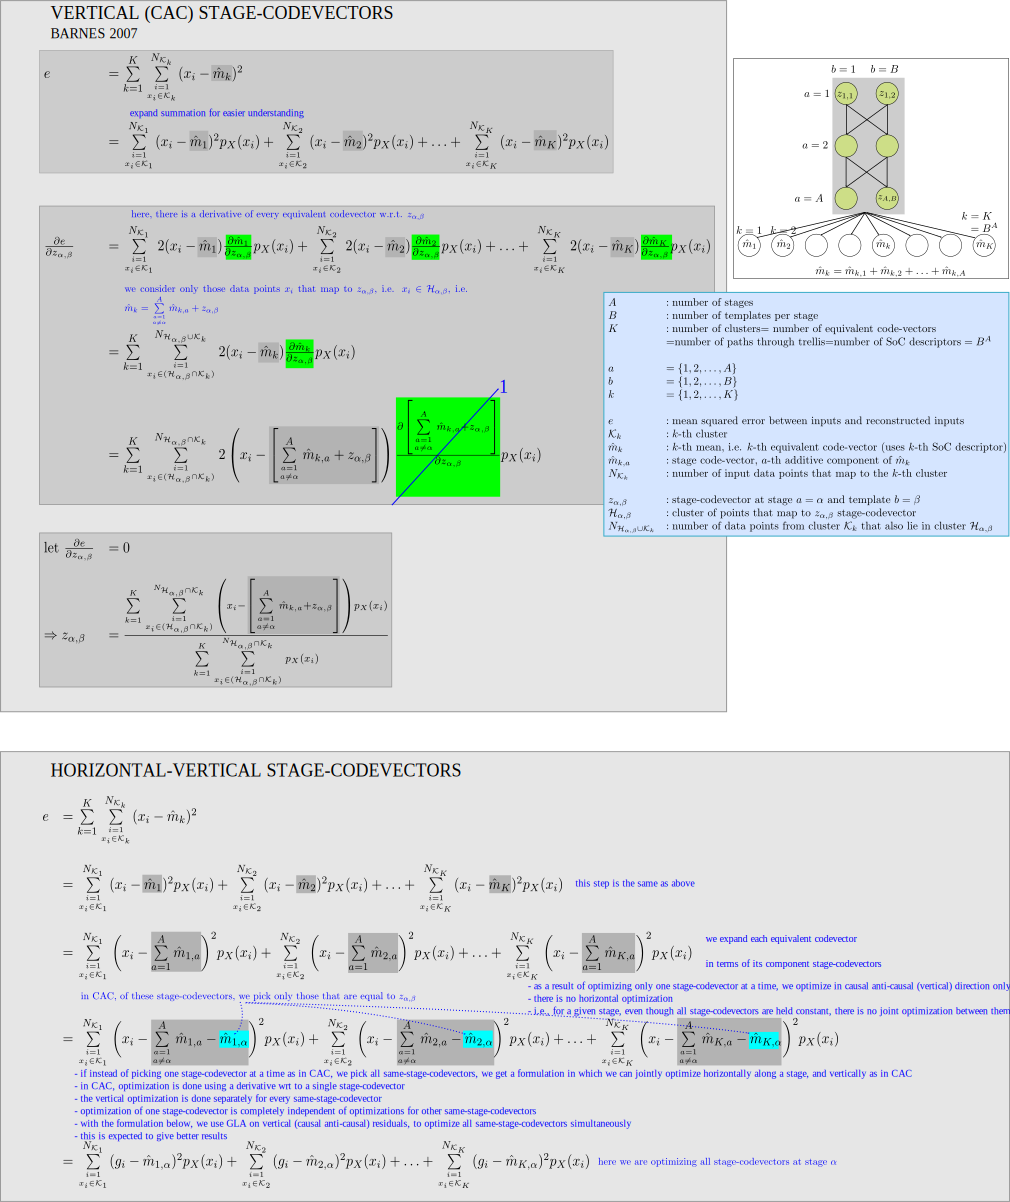
\includegraphics[width=1.0\textwidth]{figs/RVQ_CAC_derivation.pdf}
		\end{figure}
	%\end{changemargin}
\end{frame}


%=====================================
\subsection{\ \ \ \ comparison}
%=====================================

\begin{frame}[plain]
\frametitle{Introduction}
\framesubtitle{comparison with ESVQ, TSVQ}
\logoCSIPCPL\mypagenum
	\begin{changemargin}{-1.3in}{0in}
		\begin{figure}				
			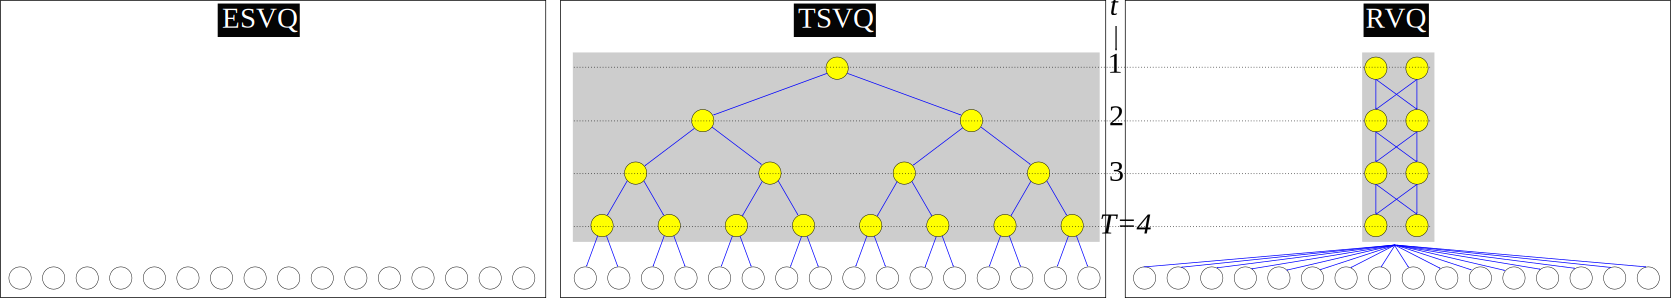
\includegraphics[width=1.3\textwidth]{figs/RVQ_comparisonWithESVQ_TSVQ.pdf}
		\end{figure}
	\end{changemargin}
\end{frame}


\begin{frame}[plain]
\frametitle{Introduction}
\framesubtitle{comparison with PCA}
\logoCSIPCPL\mypagenum
	\begin{changemargin}{-1.3in}{0in}
		\begin{figure}				
			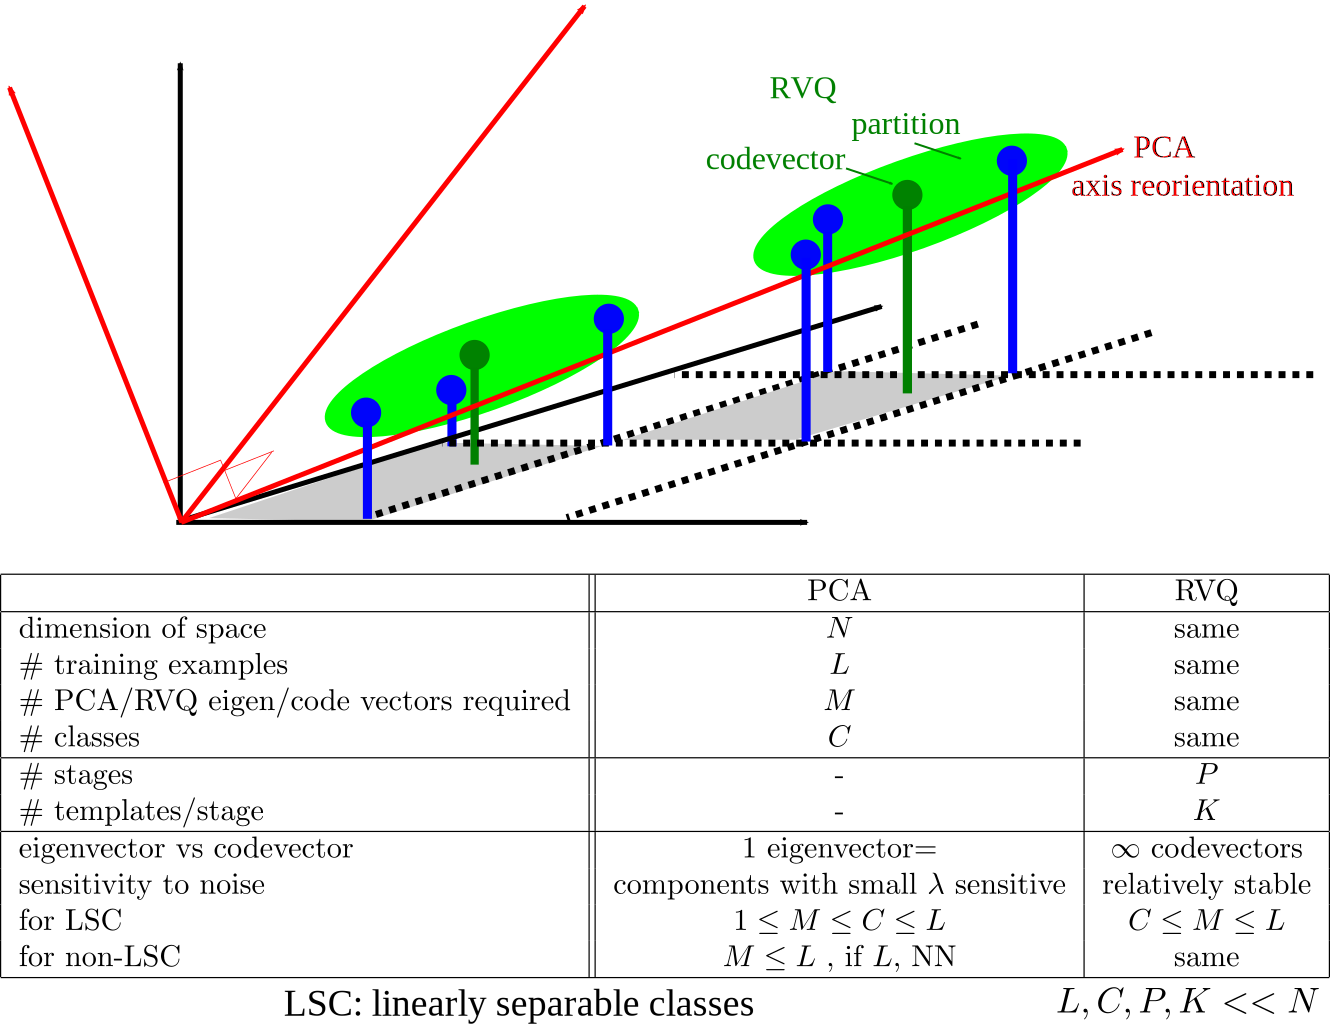
\includegraphics[height=0.8\textheight]{figs/RVQ_comparisonWithPCA.pdf}
		\end{figure}
	\end{changemargin}
\end{frame}




\begin{frame}
\frametitle{Introduction}
\framesubtitle{comparison with PCA (cont.)}
\mypagenum
	\begin{itemize}
		\item in this example, LSC, $N$ = $L$ = $C$=3,
			\begin{itemize}
				\item here, M = $C-1$, but in general will be $\leq C$
				\item same result even if $N>>L, C$
				\item practical scenarios: $N>>L>C$
				\item $L$=$C$ considered here is worse case scenario
			\end{itemize}
	\end{itemize}
\logoCSIPCPL\mypagenum	
		\multiinclude[<+>][format=pdf, start=1, graphics={width=0.8\textwidth}]{figs/PRML_PCA_simpleExample_3classes_1examplePerClass}
\end{frame}



\begin{frame}
\frametitle{Introduction}
\framesubtitle{comparison with PCA: conclusions}
	\begin{itemize}
		\item in practical scenarios, $N>>L>C$, we will get null eigenvalues for PCA
		\item however, this is ok, since all the variation is captured in eigenvectors corresponding to non-null eigenvalues
		\item in the simplest LSC case, all classes are spread across a single dimension and can be separated by eigenvalues, then for PCA, $M=1$, for RVQ, $M \geq C$
		\item in the worse LSC case, classes span the entire space, then for PCA, $M \leq C$, for RVQ, non-tight upper bound, $C \leq M \leq L$
		\item tomorrow, will generate graphic showing how 1 eigenvector = $\infty$ codevectors
	\end{itemize}
\end{frame}




%====================================
\subsection{\ \ \ \ classification methods}
%====================================
\begin{frame}
\frametitle{Introduction}
\framesubtitle{classification methods}
\logoCSIPCPL\mypagenum
	\begin{enumerate}
		\item {\color{blue} $sXDR$}
			\begin{itemize}  
				\item the class with the closest $sXDR$ is chosen
				\item "closeness" is measured using Euclidean or hamming distance
			\end{itemize}
		\item {\color{blue} $CCD$}:  
			\begin{itemize}
				\item class conditional densities are created using the $XDR$'s of a class
				\item a Naive Bayes Classifier on the $sXDR$s is used for classification
			\end{itemize}
	\end{enumerate}
\end{frame}

%========================================
\subsection{\ \ \ \ worked problems}
%========================================

\begin{frame}[plain]
\frametitle{Introduction}
\framesubtitle{worked problem 1}
\logoCSIPCPL\mypagenum
	\begin{changemargin}{-1.3in}{0in}
		\begin{figure}				
			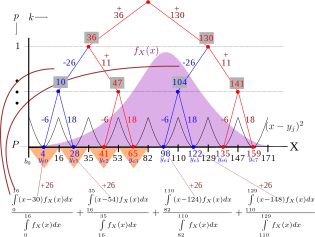
\includegraphics[width=0.9\textwidth]{figs/RVQ_stagewise_example.pdf}
			\label{fig:RVQ_SQ_DMSE}
		\end{figure}
	\end{changemargin}
\end{frame}



\begin{frame}[plain]
\frametitle{Introduction}
\framesubtitle{worked problem 2}
\logoCSIPCPL\mypagenum
	\begin{changemargin}{-1.3in}{0in}
		\begin{figure}				
			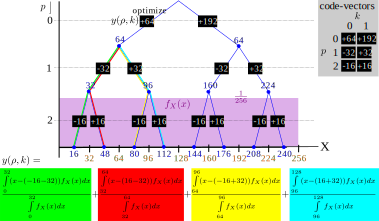
\includegraphics[width=1.0\textwidth]{figs/RVQ_stagewise_example2.pdf}
			\label{fig:RVQ_SQ_DMSE}
		\end{figure}
	\end{changemargin}
\end{frame}



%######################################################################
\section{PRIOR WORK}
%######################################################################
%============================
\subsection{\ \ \ \ Kmeans vs PCA}
%============================
\begin{frame}
\frametitle{Prior work: Kmeans vs PCA}
\framesubtitle{overview}
\mypagenum
	\begin{itemize}
		\item a
	\end{itemize}
\footnote{\tiny \myFootnoteCitation{2004_CNF_KmeansVsPCA_DingHe}{ICML}}
\end{frame}




\begin{frame}[plain]
\frametitle{Prior work: Kmeans vs PCA}
\framesubtitle{Kmeans vs PCA: step 1 (minimize intra-cluster distance)}
\mypagenum
	\begin{changemargin}{-1.35in}{0in}
		\begin{figure}
			\includegraphics[width=1.35\textwidth]{figs/PRML_PCA_Kmeans_step1.pdf}
		\end{figure}
	\end{changemargin}
\footnote{\tiny \myFootnoteCitation{2004_CNF_KmeansVsPCA_DingHe}{ICML}}
\end{frame}




\begin{frame}[plain]
\frametitle{Prior work: Kmeans vs PCA}
\framesubtitle{Kmeans vs PCA: step 2}
\mypagenum
	\begin{changemargin}{-1.35in}{0in}
		\begin{figure}
			\includegraphics[width=1.35\textwidth]{figs/PRML_PCA_Kmeans_step2.pdf}
		\end{figure}
	\end{changemargin}
\footnote{\tiny \myFootnoteCitation{2004_CNF_KmeansVsPCA_DingHe}{ICML}}
\end{frame}



\begin{frame}[plain]
\frametitle{Prior work: Kmeans vs PCA}
\framesubtitle{Kmeans vs PCA: step 3 (matrix form)}
\mypagenum
	\begin{changemargin}{-1.35in}{0in}
		\begin{figure}
			\includegraphics[width=1.35\textwidth]{figs/PRML_PCA_Kmeans_step3.pdf}
		\end{figure}
	\end{changemargin}
\footnote{\tiny \myFootnoteCitation{2004_CNF_KmeansVsPCA_DingHe}{ICML}}
\end{frame}


\begin{frame}
\frametitle{Prior work: Kmeans vs PCA}
\framesubtitle{Kmeans vs PCA: step 4 (change of cluster indicator vectors)}
\mypagenum
	\begin{figure}
		\includegraphics[width=0.6\textwidth]{figs/PRML_PCA_Kmeans_step4.pdf}
	\end{figure}
	{\tiny proof that Tr$(Q_{k-1}^TY^TYQ_{k-1})$ is maximized when $Q$ contains the eigenvectors of $Y^TY$ can be found in the geometric derivation of PCA: {\color{blue}  \href{http://users.ece.gatech.edu/~msalman/theory_3_PRML_PCA_slides.pdf}{http://users.ece.gatech.edu/\textasciitilde msalman/theory\_3\_PRML\_PCA\_slides.pdf}}}\\
	{\color{red} Conclusion}: the K-means objective function is optimized when the cluster centroid subspace is spanned by the first $K-1$ principal directions
\footnote{\tiny \myFootnoteCitation{2004_CNF_KmeansVsPCA_DingHe}{ICML}}
\end{frame}


\begin{frame}
\frametitle{Prior work: Kmeans vs PCA}
\framesubtitle{Kmeans vs PCA: conclusions}
\mypagenum
	\begin{itemize}
		\item the K-means objective function is optimized when the cluster centroid subspace is spanned by the first $K-1$ principal directions
		\item this is inherently pleasing since PCA is the optimal linear transformation to minimize mean squared error, and K-means also attempts to minimize mean squared error
	\end{itemize}
\footnote{\tiny \myFootnoteCitation{2004_CNF_KmeansVsPCA_DingHe}{ICML}}
\end{frame}


%============================
\subsection{\ \ \ \ image classification}
%============================

\begin{frame}
\frametitle{Prior Work}
\framesubtitle{\small Classification, training phase \\(Synthetic Aperture Radar: tanks)}
\logoCSIPCPL\mypagenum\footnote{Barnes, 2007}
	\begin{figure}		
		\includegraphics[height=0.30\textheight]{figs/RVQ_SARtank_1_snippets.png}			
	\end{figure}
	\begin{figure}
		\includegraphics[height=0.30\textheight]{figs/RVQ_SARtank_2_codebooks.png}
	\end{figure}
\end{frame}




\begin{frame}
\frametitle{Prior Work}
\framesubtitle{\small Classification, testing phase \\(Synthetic Aperture Radar: tanks)}
\logoCSIPCPL\mypagenum\footnote{Barnes, 2007}
	\begin{figure}		
		\includegraphics[height=0.7\textheight]{figs/RVQ_SARtank_3_reconstruction.png}			
	\end{figure}
\end{frame}




\begin{frame}
\frametitle{Prior Work}
\framesubtitle{\small Classification, training phase (Satellite imagery: pre-Tsunami Sri Lanka)}
\mypagenum\footnote{Barnes, 2007}
	\begin{figure}		
		\includegraphics[height=0.30\textheight]{figs/RVQ_SatelliteSriLanka_1_snippets.png}			
	\end{figure}
	\begin{figure}		
		\includegraphics[height=0.30\textheight]{figs/RVQ_SatelliteSriLanka_2_codebooks.png}			
	\end{figure}
\end{frame}




\begin{frame}
\frametitle{Prior Work}
\framesubtitle{\small Classification, testing phase (Satellite imagery: pre-Tsunami Sri Lanka)}
\mypagenum\footnote{Barnes, 2007}
	\begin{figure}		
		\includegraphics[height=0.4\textheight]{figs/RVQ_SatelliteSriLanka_3_labeling.png}
		\caption{\hspace{1.3in}{\color{yellow}yellow}: dirt paths \\\hspace{1.3in}{\color{blue}blue}: rivers \\\hspace{1.3in}{\color{red}red}: paved roads \\\hspace{1.3in}{\color{green}green}: train tracks}
	\end{figure}
\end{frame}



\begin{frame}
\frametitle{Prior Work}
\framesubtitle{\small Classification, training phase (Satellite imagery: Gulfport MS, post-Katrina)}
\mypagenum\footnote{Barnes, 2007}
	\begin{figure}		
		\includegraphics[width=0.7\textwidth]{figs/RVQ_SatelliteKatrina_1_snippets.png}			
	\end{figure}
	\begin{figure}		
		\includegraphics[width=0.5\textwidth]{figs/RVQ_SatelliteKatrina_2_codebooks.png}			
	\end{figure}
\end{frame}





\begin{frame}[plain]
\frametitle{Prior Work}
\framesubtitle{\small Classification, testing phase (Satellite imagery: Gulfport MS, post-Katrina)}
\mypagenum\footnote{Barnes, 2007}
	\begin{columns}
		\begin{column}{0.8in}
			\begin{changemargin}{-1.3in}{0in}
				Features detected
				\begin{enumerate}\tiny
					\item roof shingles
					\item roof edges
					\item house detections
					\item wind-damaged home locations
					\item roof damaged subfeatures
					\item grassy fields
					\item bare soils
					\item asphalt and curb subfeatures
					\item parking area
					\item train track features
					\item standing tree detections
					\item obstruction points
					\item candidate refugee sites
					\item sand deposits
					\item standing water
					\item scattered shipping containers
				\end{enumerate}
			\end{changemargin}
		\end{column}
	\begin{column}{2.8in}
			\begin{figure}		
				\includegraphics[height=0.65\textheight]{figs/RVQ_SatelliteKatrina_3_labeling.png}
			\end{figure}
			\hspace{-0.2in}
	\end{column}
	\end{columns}
\end{frame}


%####################################################################################################
\section{THEORY}
%####################################################################################################
%=======================================
\subsection{\ \ \ \ RVQ vs PCA}
%=======================================

\begin{frame}
\frametitle{Theory}
\framesubtitle{RVQ vs PCA}
\mypagenum
	\begin{itemize}
		\item {\color{red}Goal}: theoretical analysis of RVQ
		\item RVQ has many similarities with K-means clustering and PCA
			\begin{itemize}
				\item K-means \& RVQ connection: Barnes and Frost, 1992
				\item K-means \& PCA connection: Ding and He, 2004
		\end{itemize}
	\end{itemize}
	\begin{figure}
		\includegraphics[width=1.0\textwidth]{figs/RVQ_relationships.pdf}
	\end{figure}

\end{frame}



\begin{frame}
\frametitle{Theory}
\framesubtitle{RVQ vs PCA}
\logoCSIPCPL\mypagenum
	\begin{itemize}
		\item In the following slides, we use K-means and ESVQ (Exhaustive Search Vector Quantizers) interchangeably
			\begin{itemize}
				\item the reason for this is that K-means is largely used to design code-vectors (cluster means) for ESVQ
			\end{itemize}
		\item Generally, structurally constrained quantizers such as RVQ cannot provide performance as good as ESVQ
			\begin{itemize}
				\item However, RVQ can handle higher dimensions due to its linear complexity
				\item Better performance than ESVQ may therefore be possible, for given implementation cost
			\end{itemize}
	\end{itemize}
\end{frame}



\begin{frame}
\frametitle{Theory}
\framesubtitle{RVQ vs PCA: notation overview}
\mypagenum
	{\tiny also refer to notation subsection in Introduction section}
	\begin{figure}
		\includegraphics[width=1.0\textwidth]{figs/RVQ_subspaces_table.pdf}
	\end{figure}	
\end{frame}

\begin{frame}
\frametitle{Theory}
\framesubtitle{RVQ vs PCA: example}
\mypagenum
	\begin{figure}
		\includegraphics[width=1.0\textwidth]{figs/RVQ_subspaces_graphical.pdf}
	\end{figure}	
\end{frame}

\begin{frame}
\frametitle{Theory}
\framesubtitle{RVQ vs PCA: are stage codevectors independent?}
\mypagenum
	\begin{itemize}
		\item At stage 1, we have $L$ input data points which are assumed to be independent
			\begin{itemize}
				\item these data points have codevectors subtracted from them, the codevector selected for a data point is the centroid of the partition to which it belongs
				\item as a result, each input data point is shifted towards the origin, but remains independent of other data points
				\item as a result, the $M$ stage codevectors are independent from each other as well as independent of the stage codevectors of the previous stage
				\item as a result, the $M-1$ principal directions of each stage are independent
			\end{itemize}
	\end{itemize}	
\end{frame}



\begin{frame}[plain]
\frametitle{Theory}
\framesubtitle{RVQ vs PCA (cont.)}
\mypagenum
	\begin{changemargin}{-1.4in}{0in}
		\begin{figure}
			\includegraphics[width=1.4\textwidth]{figs/RVQ_subspaces_comments.pdf}
		\end{figure}	
	\end{changemargin}
\end{frame}


\begin{frame}[plain]
\frametitle{Theory}
\framesubtitle{RVQ vs PCA (cont.)}
\mypagenum
	\begin{changemargin}{-1.4in}{0in}
		\begin{figure}
			\includegraphics[width=1.4\textwidth]{figs/RVQ_subspaces_comments2.pdf}
		\end{figure}	
	\end{changemargin}
\end{frame}




\begin{frame}
\frametitle{Theory}
\framesubtitle{RVQ vs PCA (cont.)}
\mypagenum
	\begin{itemize}
		\item so, why RVQ?
			\begin{itemize}
				\item 
			\end{itemize}
	\end{itemize}
\end{frame}


%####################################################################################################
\section{METHODOLOGY}
%####################################################################################################
%\begin{frame}
%\frametitle{Methodology}
%\logoCSIPCPL\mypagenum
%\href{run:distribute/RVQ_tracking.bat}{{\color{blue}\underline {Click to view video on RVQ tracking}}}
%\end{frame}
%
%
%\begin{frame}
%\frametitle{Methodology}
%\logoCSIPCPL\mypagenum
%\href{run:distribute/RVQ_Entire_process_PSNR_creation.bat}{{\color{blue}\underline {Click to view video on RVQ tools}}}
%\end{frame}


\begin{frame}
\frametitle{Methodology}
\framesubtitle{}
%\logoCSIPCPL\mypagenum
\includemovie[ poster, text=(click to play video), mouse, repeat ]{ 1.0\linewidth }{ .75\linewidth }{distribute/RVQ_Entire_process_PSNR_creation_part1.MP4} 
\end{frame}


\begin{frame}
\frametitle{Methodology}
\framesubtitle{}
%\logoCSIPCPL\mypagenum
\includemovie[ poster, text=(click to play video), mouse, repeat ]{ 1.0\linewidth }{ .75\linewidth }{distribute/RVQ_Entire_process_PSNR_creation_part2.MP4} 
\end{frame}


\begin{frame}
\frametitle{Methodology}
\framesubtitle{}
%\logoCSIPCPL\mypagenum
\includemovie[ poster, text=(click to play video), mouse, repeat ]{ 1.0\linewidth }{ .75\linewidth }{distribute/RVQ_tracking.MP4} 
\end{frame}




%####################################################################################################
\section{EXPERIMENTS}
%####################################################################################################

%====================================
\subsection{\ \ \ \ image classification}
%====================================




\begin{frame}
\frametitle{Experiments}
\framesubtitle{dataset used: sample images}
\logoEvolution\mypagenum	
	\begin{figure}
		\includegraphics[width=1.0\textwidth]{figs/PRML_PCA_faceRecognition_1_trainingFaces.png}
	\end{figure}
\end{frame}

\begin{frame}
\frametitle{Introduction}
\framesubtitle{dataset used}
\logoCSIPCPL\mypagenum
	\begin{itemize}
		\item Yale face dataset
		\item Number of different classes (i.e. persons): 15
		\item Number of examples/class (i.e. images/person): 11
		\item Total number of images: 15x11=165
		\item Original image size: 159x159
		\item Images resized to: 63x63
		\item {\color{red}Attention: For RVQ, inner 51x51 pixels used}
	\end{itemize}
\end{frame}


\begin{frame}
\frametitle{Experiments}
\framesubtitle{overall procedure for RVQ, SVM and PCA}
\logoCSIPCPL\mypagenum
	\begin{itemize}
		\item {\color{red}Cross-validation} used
			\begin{enumerate}
				\item First image selected as test image
				\item Training done with remaining images
					\begin{itemize}
						\item for Yale dataset which has 165 images, training done with remaining 164 images
					\end{itemize}
				\item Test image classified using training model
				\item Second image selected as test image
				\item Training done with remaining images
				\item Test image classified using training model
				\item and so on for all images in dataset
			\end{enumerate}
	\end{itemize}
\end{frame}



\begin{frame}
\frametitle{Experiments}
\framesubtitle{RVQ experimental procedure}
\logoCSIPCPL\mypagenum	
	\begin{enumerate}
		\item Pre-processing
			\begin{enumerate}[(a)]
				\item grayscale images converted to 6 channel (pos-neg)
				\item center of image chosen: 51x51 (snippet size)
			\end{enumerate}
		\item Training
			\begin{enumerate}[(a)]
				\item experimenting with codebook generation parameters
				\item training with codebooks
				\item generation of $sXDR$'s for codebook images
				\item generation of class conditional densities using codebook images
			\end{enumerate}
		\item Testing
			\begin{enumerate}[(a)]
				\item classification using euclidean distance on $sXDR$'s
				\item classification using hamming distance on $sXDR$'s
				\item classification using Naive Bayes Classifier
			\end{enumerate}
	\end{enumerate}
\end{frame}



\begin{frame}
\frametitle{Experiments}
\framesubtitle{RVQ training: experimenting with codebook generation parameters}
\mypagenum	
		\begin{itemize}
			\item the goal was to see what SNR value results in how many number of stages, and to see how codebook appearances change with increasing SNR values
			\item all 165 images were used
			\item the next few slides elaborate on this, to see what the codebooks actually look like, see {\color{blue}  \href{http://users.ece.gatech.edu/~msalman/distribute/theory_3_PRML_RVQ_extensiveTraining.pdf}{this}}
		\end{itemize}
\end{frame}



\begin{frame}
\frametitle{Experiments}
\framesubtitle{RVQ training: experimenting with codebook generation parameters (cont.)}
\mypagenum
	\begin{itemize}
		\item In order to understand how codebooks change with different target SNR values,
			\begin{itemize}
				\item codebooks were generated for templates/stage (TPS) going from 2 to 16 using all the images (165 in all)	
				\item target SNRs used were 0:0.2:39.8 dB (i.e. 200 distinct values)
				\item number of times RVQ trained with 165 images: 15 distinct TPS values x 200 SNR values/TPS =3000
				\item number of snippets processed=3000 training cycles x 165 snippets/cycle=495,000
				\item number of pixels processed=495,000 snippets x (51x51) pixels=1,287,495,000
				\item time taken: 72 hours
			\end{itemize}
	\end{itemize}
\end{frame}



\begin{frame}
\frametitle{Experiments}
\framesubtitle{RVQ training: experimenting with codebook generation parameters (cont.)}
\mypagenum
	In the following slide	
		\begin{itemize}
			\item notice that achieved SNR is always greater than target SNR
			\item also, achieved SNR increases smoothly and monotonically with increasing $M$ and $P$
			\item in general, a given DOF produces about the same MSE, for example, 8x2 produces SNR=13 dB, which is equal to that produced by 4x4 and 2x8 
		\end{itemize}
\end{frame}



\begin{frame}
\frametitle{Experiments}
\framesubtitle{RVQ training: experimenting with codebook generation parameters (cont.)}
\mypagenum	
	\multiinclude[<+>][format=jpg, start=1, end=8, graphics={height=0.5\textheight}]{figs/new/RVQ_yaleFaces_dcbk_M_2}
\end{frame}



\begin{frame}
\frametitle{Experiments}
\framesubtitle{RVQ training: experimenting with codebook generation parameters (cont.)}
\mypagenum	
	\multiinclude[<+>][format=jpg, start=1, end=8, graphics={height=0.5\textheight}]{figs/new/RVQ_yaleFaces_dcbk_M_3}
\end{frame}


\begin{frame}
\frametitle{Experiments}
\framesubtitle{RVQ training: experimenting with codebook generation parameters (cont.)}
\mypagenum	
	\multiinclude[<+>][format=jpg, start=1, end=8, graphics={height=0.5\textheight}]{figs/new/RVQ_yaleFaces_dcbk_M_4}
\end{frame}


\begin{frame}[plain]
\frametitle{Experiments}
\framesubtitle{RVQ training: experimenting with codebook generation parameters (cont.)}
\mypagenum
	\begin{changemargin}{-0.7in}{0in}	
		\begin{figure}
			\includegraphics[width=0.4\textwidth]{figs/RVQ_yaleFaces_dcbk_dSNR.pdf}
		\end{figure}
		\tiny SNR targeted
		\begin{tiny}
		\input{tables/RVQ_yaleFaces_dcbk_dSNR_target} 
		\end{tiny}		
		\tiny SNR achieved
		\begin{tiny}
		\input{tables/RVQ_yaleFaces_dcbk_dSNR_achieved} 
		\end{tiny}
	\end{changemargin}
\end{frame}


\begin{frame}
\frametitle{Experiments}
\framesubtitle{RVQ training: generating $sXDR$'s}
\logoCSIPCPL\mypagenum
	In the following slides,
	\begin{itemize}
		\item we show values of $sXDR$'s for training images (164 in all since one test image has been taken out) 
		\item classes should have a non-overlapping range of amplitude values
		\item we fix $P=8$
		\item the 164 training images have been colored {\color{blue}manually} according to class
			\begin{itemize}
				\item the goal is to be able to do this {\color{blue}automatically} using the decimal p-tuple
				\item images of a class are drawn together (total of 15 users, i.e. classes) so that intra-class variation can be better viewed
				\item different classes may have the same color since there are not enough colors to give each class a separate color
			\end{itemize}
	\end{itemize}
\end{frame}




%\begin{frame}
%\frametitle{Experiments}
%\framesubtitle{RVQ decimal p-tuples: \small $x_i=\sum_{p=0}^{P-1}XDR(p)u^{(P-1-p)}$}
%\mypagenum
%	\multiinclude[<+>][format=pdf, start=2, end=8, graphics={width=1.0\textwidth}]{figs/RVQ_yaleFaces_decimal_ptuples_combined_M}
%\item See effects of changing $u$ on a single slide and changing $M$ from slide to slide
%\item For a particular value of M, we try different values of the geometric weights, $u=1,2,3,4,5,6,7,8$
%\item $u=M$ should be used since this setting is invertible, nevertheless, we show all values of $u$
%\item intra-class variation decreases with increasing $u$ 
%\item inter-class variation decreases with increasing $M$
%\end{frame}



\begin{frame}
\frametitle{Experiments}
\framesubtitle{RVQ training: generating $sXDR$'s}
\mypagenum
	\multiinclude[<+>][format=pdf, start=2, end=8, graphics={width=0.7\textwidth}]{figs/RVQ_yaleFaces_decimal_ptuples_M}
	\\{\tiny Invertible mapping between $XDR$ and $sXDR$, $sXDR =\sum\limits_{t=1}^{T}\mathbf{i}(t)S^{(T-t)}$.  $M$ is the number of stages.  The x-axis goes from 0 to 163 for the 164 images.  The y-axis is the value of the $sXDR$.}
\end{frame}


\begin{frame}
\frametitle{Experiments}
\framesubtitle{RVQ training: generating CCD's}
	\begin{itemize}
		\item we have few examples per class
		\item options to generate a density
			\begin{itemize}
				\item {\color{blue}fit gaussian}: not used
				\item {\color{blue}kernel density estimation}: not used
				\item {\color{blue}normalized histogram}: $XDR$ histogram generated, empty bins were given a small value $\delta$, and the histogram was normalized to create a density 
			\end{itemize}
	\end{itemize}
\logoCSIPCPL\mypagenum
\end{frame}


\begin{frame}
\frametitle{Experiments}
\framesubtitle{PCA: experimental procedure}
\logoEvolution\mypagenum	
	\begin{enumerate}
		\item Training
			\begin{enumerate}[(a)]
				\item generation of eigenfaces
			\end{enumerate}
		\item Testing
			\begin{enumerate}[(a)]
				\item projection of test image onto eigenfaces
				\item retention of $q$ projections
				\item classification using euclidean distance on $q$ projections
			\end{enumerate}			
	\end{enumerate}
\end{frame}



\begin{frame}
\frametitle{Experiments}
\framesubtitle{PCA: average training face}
\logoEvolution\mypagenum	
	\begin{figure}
		\includegraphics[width=0.5\textwidth]{figs/PRML_PCA_faceRecognition_3_averageFace.png}
	\end{figure}
\end{frame}


\begin{frame}
\frametitle{Experiments}
\framesubtitle{PCA: eigenfaces}
\logoEvolution\mypagenum	
	\begin{figure}
		\includegraphics[width=1.0\textwidth]{figs/PRML_PCA_faceRecognition_6_eigenFaces.png}
	\end{figure}
\end{frame}


\begin{frame}
\frametitle{Experiments}
\framesubtitle{PCA: sample reconstruction}
\logoEvolution\mypagenum	
	\begin{figure}
		\includegraphics[width=1.0\textwidth]{figs/PRML_PCA_faceRecognition_9_reconstruction.png}
	\end{figure}
\end{frame}


\begin{frame}
\frametitle{Experiments}
\framesubtitle{SVM: experimental procedure}
\mypagenum
	In the following slides, we perform a grid search over $C$ and $\gamma$ for different SVM kernels to find best classification performance
	\begin{itemize}
		\item {\color{blue}x axis:} $C \in \{2^{-5}, 2^{-4} \ldots 2^{15}\}$, 21 distinct points
		\item {\color{blue}y axis:} $\gamma \in \{2^{-15}, 2^{-14} \ldots 2^{3}\}$, 19 distinct points
		\item {\color{blue}total points searched:} 21 x 19 = 399
	\end{itemize}
\end{frame}



\begin{frame}[plain]
\frametitle{Experiments}
\framesubtitle{SVM kernels: grid search over $C$ and $\gamma$}
\mypagenum
	\begin{changemargin}{-1.3in}{0in}
		\begin{figure}
			\centering
			\subfigure
			{
				\includegraphics[width=0.3\textwidth]{figs/SVM_yaleFace_linearKernel_3Dsurf.pdf}
			}
			\subfigure
			{
				\includegraphics[width=0.3\textwidth]{figs/SVM_yaleFace_polynomialKernel_3Dsurf.pdf}
			}
			\subfigure
			{
				\includegraphics[width=0.3\textwidth]{figs/SVM_yaleFace_RBFkernel_3Dsurf.pdf}
			}
			\subfigure
			{
				\includegraphics[width=0.3\textwidth]{figs/SVM_yaleFace_sigmoidKernel_3Dsurf.pdf}
			}
			\subfigure
			{
				\includegraphics[width=0.3\textwidth]{figs/SVM_yaleFace_linearKernel_2D.pdf}
			}
			\subfigure
			{
				\includegraphics[width=0.3\textwidth]{figs/SVM_yaleFace_polynomialKernel_2D.pdf}
			}
			\subfigure
			{
				\includegraphics[width=0.3\textwidth]{figs/SVM_yaleFace_RBFkernel_2D.pdf}
			}	
			\subfigure
			{
				\includegraphics[width=0.3\textwidth]{figs/SVM_yaleFace_sigmoidKernel_2D.pdf}
			}	
			\caption{L to R, kernels: linear (90\%), polynomial (83\%), RBF (90\%), sigmoid (93\%), top row contains 3D plots, bottom row contains corresponding 2D plots}
		\end{figure}
	\end{changemargin}
\end{frame}


\begin{frame}
\frametitle{Experiments}
\framesubtitle{SVM kernels: grid search over $C$ and $\gamma$}
\mypagenum
	\begin{figure}
		\centering
		\subfigure[Linear kernel: 90\%]
		{
			\includegraphics[width=0.40\textwidth]{figs/SVM_yaleFace_linearKernel_hist.pdf}
		}
		\subfigure[Polynomial kernel: 83\%]
		{
			\includegraphics[width=0.40\textwidth]{figs/SVM_yaleFace_polynomialKernel_hist.pdf}
		}
		\subfigure[RBF kernel: 90\%]
		{
			\includegraphics[width=0.40\textwidth]{figs/SVM_yaleFace_RBFkernel_hist.pdf}
		}
		\subfigure[Sigmoid kernel: 93\%]
		{
			\includegraphics[width=0.40\textwidth]{figs/SVM_yaleFace_sigmoidKernel_hist.pdf}
		}
		\caption{\tiny Classification accuracies for different combinations of $C$ and $\gamma$.  Notice that the polynomial kernel gives 82\% classification accuracy over several combinations of $C$ and $\gamma$}
	\end{figure}
\end{frame}



%####################################################################################################
\section{RESULTS}
%####################################################################################################
%====================================
\subsection{\ \ \ \ image classification}
%====================================

\begin{frame}
\frametitle{Results}
\framesubtitle{RVQ: classification accuracy \%}
\logoCSIPCPL\mypagenum
	\begin{figure}
		\includegraphics[width=0.5\textwidth]{figs/RVQ_yaleFace_classifications.pdf}
	\end{figure}
	{\tiny NB: Naive Bayes Classifier}\\
	\center{\input{tables/RVQ_yaleFaces_classification}\\
	{\color{red} Highest classification accuracy achieved: 72\%}}
\end{frame}


\begin{frame}
\frametitle{Results}
\framesubtitle{PCA: classification accuracy \%}
\logoCSIPCPL\mypagenum	
	\begin{figure}
		\includegraphics[width=1.0\textwidth]{figs/PCA_comparison.pdf}
	\end{figure}
	{\color{red} Highest classification accuracy achieved: 79\%}
\end{frame}


\begin{frame}
\frametitle{Results}
\framesubtitle{SVM: classification accuracy \%}
\logoCSIPCPL\mypagenum
	\begin{itemize}
		\item Linear kernel: 90\%
		\item Polynomial kernel: 83\%
		\item RBF kernel: 90\% 
		\item Sigmoid kernel: 93\%
	\end{itemize}
	{\color{red} Highest classification accuracy achieved: 93\%}
\end{frame}




%####################################################################################################
\section{CONCLUSIONS}
%####################################################################################################
%====================================
\subsection{\ \ \ \ image classification}
%====================================
\begin{frame}
\frametitle{Conclusions}
\framesubtitle{}
\logoCSIPCPL\mypagenum
	\begin{itemize}
		\item {\color{red}RVQ}
			\begin{itemize}
				\item Highest classification accuracy is 72\%
				\item Classification results are expected to improve after using more stages
			\end{itemize}
		\item {\color{red}PCA}
			\begin{itemize}
				\item Only around 40 eigenvectors out of 165 are needed to achieve the highest classification possible, i.e. 79\%
			\end{itemize}
		\item {\color{red}RVQ vs PCA}
			\begin{itemize}
				\item RVQ using 8 stages and PCA using 8 codevectors have nearly the same classification accuracy (72\% vs 73\% respectively)
			\end{itemize}
		\item {\color{red}SVM} 
				\begin{itemize}
					\item Performance for linear, RBF and sigmoid kernels is around the same, i.e. around 90\%	
				\end{itemize}
		\item {\color{red}Overall} 
			\begin{itemize}
				\item The best classification result is for SVM (sigmoid kernel) at 93\%	
			\end{itemize}
	\end{itemize}
\end{frame}


%####################################################################################################
\section{FUTURE WORK}
%####################################################################################################
\begin{frame}
\frametitle{Future work}
\framesubtitle{}
\logoCSIPCPL\mypagenum
	\begin{itemize}
		\item Theory
			\begin{itemize}		
				\item bounds on generalization error
			\end{itemize}
		\item Experiments
			\begin{itemize}
				\item start working with tracking datasets
			\end{itemize}
	\end{itemize}
\end{frame}




%####################################################################################################
\printbibliography
%####################################################################################################
%\bibliographystyle{ieee}
%\bibliography{c:/salman/work/writing/MyCitations}
\end{document}
%####################################################################################################

%####################################################################################################




%A VQ with a direct sum structure
%A vector quantiz
%
%
%
%\cite{Barnes_96_AdvRVQ}
%
%
%$p$th stage of an RVQ:
%
%\begin{equation}
%Q_p = R^k \mapsto C_p
%\end{equation}
%
%$R^k$ is the $k$-dimensional input space of each RVQ encoder stage, $p \in {1, 2, ... P}$ is a stage index.  $C_p = {y_p(0), y_p(1), ... y_p(N-1)}$ is the $p$th stage codebook.  $y_p(i_p) \in R^k$ is a $p$th stage codevector, and $i_p$ is an index in the $p$th stage index set $I_p = {0,1,... N_p-1}$   
%
%Type I encoder: \\
%Input vector is compared with a certain threshold.  If it exceeds it, it is encoded.  The residual is then compared with another threshold, and so on.
%
%Type II encoder: \\
%A vector goes straight to a level where it should be encoded.
%
%%============================================================
%\subsection{Efficiences}
%%============================================================
%Dimensions: n\\
%Stage residual templates: M\\
%Number of levels: P
%
%Computation (search) and memory (storage) requirements are proportional to $n x M x P$.  So, cost functional grows linearly with classifier dimensionality $n$, branch multiplicity $M$, and the number of tree levels $P$.  A near neighbor search is proportional in computational complexity to $MP$ whereas there is one of $M^P$ possible outcomes.
%
%%============================================================
%\subsection{Pattern Matching}
%%============================================================	
%
%%============================================================   
%\subsection{Kinds of trees}
%%============================================================
%In graph theory, a tree is a connected acyclic graph. 



%David Newhoff

%\begin{frame}
%\frametitle{RVQ}
%\framesubtitle{optimality}
%\logoCSIPCPL\mypagenum
%	\begin{itemize}
%		\item {\color{red}$\rho$}: vertical index
%			\begin{itemize}
%				\item index of the codebook that we're optimizing, $\rho \in \{1, 2, ... , P\}$
%			\end{itemize}
%		\item {\color{red}$k$}: horizontal index 
%			\begin{itemize}
%				\item codevector index at a particular level $p$
%			\end{itemize}
%		\item {\color{red}$j_P$}: $p$-tuple.  
%			\begin{itemize}
%				\item summing over all $p$-tuples, i.e. all $j_P$, is equivalent to summing over the equivalent code-vectors
%			\end{itemize}
%		\item We want to minimize $D_{MSE}$ wrt the $k$-th codevector in $A_{\rho}$, i.e. $y_k^{\rho}$
%			\begin{itemize}
%				\item Codebooks at all levels are fixed, except the $\rho$-th level, i.e., $A_{\rho}$
%				\item {\color{red}$H_k^{\rho}$} is the set of all direct sum quanta $y^e(j_P)$  that contain $y_k^{\rho}$ in their construction
%				\item Instead, we sum over a subset of the $p$-tuples, $H_k^{\rho}$
%			\end{itemize}
%	\end{itemize}
%\end{frame}




%%######################################################################
%\subsection{Notation}
%%######################################################################
%\begin{frame}\frametitle{Notation}\framesubtitle{VQ with Direct Sum Codebooks (Barnes, 1993)}\logoCSIPCPL\mypagenum
%	\begin{itemize}\tiny
%		\item {\color{red}$p$:} stage index, {\color{red}$P$:} total number of stages
%		\item {\color{red}$J^p$:} index set, $J^p = \{0, 1, \ldots N^p-1\}$, {\color{red}$j^p$:} template index, member of $J^p$ 
%			\begin{itemize}\tiny
%				\item my notation: don't use $J^p$ at all, change $j^p$ to $j$ and say $j = \{0, 1, \ldots N^p-1\}$
%			\end{itemize}
%		\item {\color{red}$\mathbf{j}^P$:} a p-tuple, product codeword, $\mathbf{j}^P = \{j^1, j^2, \ldots, j^P\}$, element of the Cartesian product of the stagewise index sets $j^P \in J^1 x J^2 x \ldots x J^P$
%		\vspace{0.15in}
%		\item input: {\color{red}$x^1$}, source vector
%		\item output: {\color{red}$y^p_{j_p}$}, stage-wise code-vectors
%		\item $p$-th stage
%		\begin{itemize}\tiny
%			\item {\color{red}$N^p$}, number of code-vectors in $A^p$ and cells in $P^p$
%			\item {\color{red}$x^p$}, residual vector, a realization of {\color{red}$X^p$}, {\color{red}$F_{X^1, X^2, \ldots, X^p}$} is the joint distribution of $X^1, X^2, \ldots, X^p$
%			\vspace{0.15in}
%			\item {\color{red}$A^p$}, set of code-vectors, $A^p = \{y^p_0, y^p_1, \ldots, y^p_{N^p-1}\}$
%			\item {\color{red}$P^p$}, partition, $P^p = \{S^p_0, S^p_2, \ldots, S^p_{N^p-1}\}$
%			\item {\color{red}$Q^p$}, quantizer, $Q^p: R^n \mapsto A^p$, $Q^p(x^p) = y^p_{j^p}$, iff $x^p \in S^p_{j^p}$
%		\end{itemize}
%		\vspace{0.15in}
%		\item {\color{red}$A^e$}, set of all possible sums of stagewise code-vectors, $A^e = A^1 + A^2 + \ldots A^P$.  There are $N^e$ such possible combinations, where $N^e=\bigcap_{p=1}^PN_P$
%		\item {\color{red}$P^e$}
%		\item {\color{red}$Q^e$}
%	\end{itemize}	
%\end{frame}





%%=============================================================
%\subsection{from older ppt}
%%=============================================================
%Joint design methods: Barnes and Frost, Chan and Gersho
%Product Code
%1. Mean residual	
%2. Gain shape
%3. Mean-gain shape
%4. RVQ
%
%Structured:
%Tree (TSVQ)
%Classified
%Transform
%Product Code
%Partitioned
%Mean removed
%Shape gain
%Multi stage
%Constrained storage
%Hierarchical and multiresolutional
%Nonlinear interpolative
%Lattice codebook
%Fast NN
%Predictive
%Finite state
%Tree and trellis
%Adaptive
%Variable rate
%
%Unstructured:
%NN
%Lattice (codebook is a lattice)




%%%=============================================================
%\subsection{Equivalent quantizer}
%%%=============================================================
%\begin{frame}\frametitle{Equivalent quantizer}\logoCSIPCPL\mypagenum
%	\begin{itemize}
%		\item Single stage equivalent quantizer	
%		\item Residual and equivalent quantizer produce same average distortion
%		\item Advantage: expected distortion in terms of $F_{x_1}$ rather than $F_{x_1 \ldots x_P}$
%		\item Equivalent codebook, equivalent mapping, equivalent partition
%	\end{itemize}
%	\begin{equation*}
%		Q_e(x^1) = \sum_{p=1}^{P}Q_p(x_p)
%	\end{equation*}
%\end{frame}

